%\chapter*{Введение}
%\addcontentsline{toc}{chapter}{Введение}

\newpage
\begin{center}
	\textbf{АННОТАЦИЯ}
\end{center}
%\refstepcounter{chapter}
\addcontentsline{toc}{chapter}{АННОТАЦИЯ}

В рамках данной работы рассматривается разработка прототипа четырехногого шагающего робота с восемью степенями свободы, а также создание для него программного обеспечения, которое включает в себя:
\begin{enumerate} 
	\item Решение задачи траекторного движения на основе численного решения обратной задачи кинематики.
	\item Моделирование и сборка физической единицы  робота.
	\item Отладка протоколов связи между контролером и серводвигателями.
	\item Отладка протоколов связи между контролером и гироскопом акселерометром.
	\item Корректирование движения робота с учетом обратной связи.
\end{enumerate}
Конечный результат представлен в виде собранного физического прототипа шагающего робота с возможностью дистанционного управления. 


\onehalfspacing
\setcounter{page}{2}
\renewcommand{\contentsname}{\centerline{\Large{Cодержание}}}
\tableofcontents
\addtocontents{toc}{\protect\thispagestyle{fancy}}
\renewcommand{\contentsname}{\centerline{\Large{Cодержание}}}

\newpage
\begin{center}
	\textbf{ВВЕДЕНИЕ}
\end{center}
%\refstepcounter{chapter}
\addcontentsline{toc}{chapter}{ВВЕДЕНИЕ}

Особенное место в робототехнике занимает подкласс шагающих роботов. Шагающими роботами принято называть класс роботов, которые имитируют походку людей или животных. Данный вид появился не просто так, их главной особенностью является как особенность походки, так и в принципе уникальная модель движения. Она позволяет быстро и, что главное, эффективно приспосабливаться к работе в неровных поверхностях. По сути, оптимизация движения шагающих роботов является главной проблемой всех ведущих исследователей в данной области. Все известные производители шагающих роботов не используют четко описанные законы движения для управления в своих продуктах. Вместо этого, они используют заранее сформированные модели глубокого обучения, основанные на больших пластах информации, собранной с реальных экземпляров. Например, для управления (обучения) четырехногих шагающих роботов использовали массивы данных, полученных с датчиков, которые в свою очередь были закреплены на собаке, схожей по физическим размерам конечностей и тела. Такие методы, как правило показывают себя более выгодными как с точки зрения точности позиционирования робота, скорости адаптации в окружении, так и выигрывают по энергоэффективности в сравнении с классическими методами, но имеют существенный недостаток в скорости разработки и в особенности требуют больших денежных затрат. 
\newpage
\textbf{Актуальность}


Задача разработки шагающих роботов не теряет актуальности по сей день. Начиная с 2004 года, когда Boston Dynamics впервые представила четырехногого шагающего робота BigDog, промышленность в данной области не сбавляет обороты и постоянно вносит новые технологии, методики в разработку, а также находит новые применения данным роботам. Прогресс можно заметить при сравнении с современными моделями Boston Dynamics или, например LaikaGo и Strelka от UniTree  (рисунок \ref{dogs}), которые используют на кафедре робототехники в МГТУ им. Н. Э Баумана.
\begin{figure}[h]
	\begin{center}
		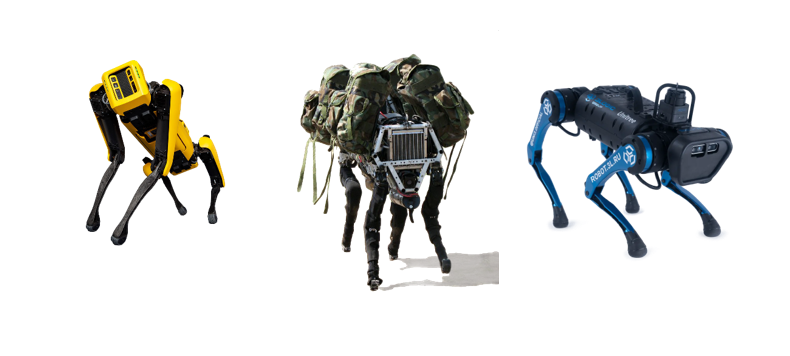
\includegraphics[width=1\textwidth]{dogs}
		\caption{BigDog и Spot от Boston Dynamics, Laika от UniTree.}
		\label{dogs}
	\end{center}
\end{figure}

Сегодня такие мобильные роботы используются для составления строительных планов здания по технологии BIM (рисунок \ref{zavod}), отслеживания хода строительства на площадках Pomerlau, а также на заводах Ford. Такие продукты стали востребованы для мониторинга оборудования в опасных условиях, например, нефтепромышленная компания AkerBP использовала робота Spot для снятия показаний и отслеживания утечек на судне FPSO в Норвегии.

\newpage
\begin{figure}[h]
	\begin{center}
		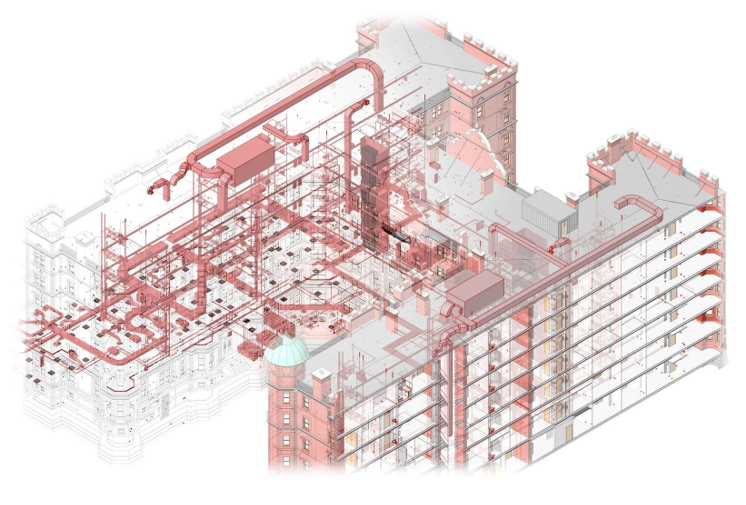
\includegraphics[width=1\textwidth]{zavod}
		\caption{Строительный план по технологии BIM.}
		\label{zavod}
	\end{center}
\end{figure}